\documentclass{article}
\usepackage[utf8]{inputenc}
\usepackage{graphicx}

\title{Data Mining Project}
\author{James Harrison}
\date{April 2022}

\begin{document}

\begin{titlepage}
   \begin{center}
       \vspace*{1cm}

       \textbf{Naive Bayesian Classification on Spam}
     
       \vspace{0.5cm}
        An Analysis on Metacritic User Score Data
            
       \vspace{1.5cm}

       \textbf{James Kyle Harrison}

       \vfill
        
            
       \vspace{0.8cm}
     
            
       Georgia Southern University\\
       April 25th, 2022
            
   \end{center}
\end{titlepage}

\section{Introduction}
\hspace{\parindent} Metacritic is a website dedicated to taking review scores from as many review publications as possible and generating an aggregate Metascore for various releases through many types of entertainment mediums. Not only does Metacritic create a Metascore for review publications, but they also allow for users to write reviews and score items on the website and it will generate an aggregate Metascore for the user reviews as well. When Metacritic first started up in the early 2000s it found success through generating these Metascores with books and movies being the most popular forms of releases being viewed, however as public interests have changed and technology has become more optimized the most popular form of entertainment (and most popular section of Metacritic) has become video games. Along with this growth of technology, and Metacritic as an entity, many more users came to the website to not only view the publication scores, but to also leave their own user reviews. Although the publication Metascore and user Metascores are separate one would think that the two aggregate scores would still be similar, however this is typically not the case. Not every user will agree with the Metascores that they see for particular titles, and as a result will sway the Metascore to however they like through a phenomenon known as review bombing. Although Metacritic tries their best to mitigate these sorts of problems, many of the users (and bots) that attempt to review bomb make it through the cracks of their security. With these sorts of influences occurring on the user reviews Metascore it is hard to make an accurate comparison to the critic Metascore.\\
\par In order to create a more fair comparison between the two Metascores one must be able to detect these fraud reviews, and remove them from the generation of the user Metascore. This document investigates the parameters and features required to create a more accurate Metascore through a classification analysis by removing these reviews and regenerating the Metascore using two public Metacritic video games datasets; a 12.1MB Metacritic video game dataset labeled as 'Top Video Games 1995-2021 Metacritic' by user Deep Contractor that has the aggregate Metascore of user and critic reviews, and Dahlia's 265MB dataset containing a list of user reviews and comments used in these reviews for the most popular games on Metacritic. Deep Contractor's dataset has occasional updates to it to add more games to the dataset as more releases occur, so to keep consistency throughout this process this document will be exploring version 4 of this dataset, whereas Dahlia's dataset does not have consistent updates. For clarification we will be running version 4 of Dahlia's dataset as well. To go along with this, there needs to be some sort of way to decide what reviews can be considered legitimate or not. To do this, we will use a third dataset, a 14.8MB review dataset labeled 'Fake Reviews Dataset' (created by Joni Salminen), to create this comparison. This dataset is a collection of 40,432 reviews that have been already been determined to rather be legitimate or not (with a little over 20,000 reviews splitting into each of the two categories), which will be important to creating this supervised implementation. \\
\par Although a significant amount of the data in these data sets are relevant to each other there are a few factors in regards to this information that need to be acknowledged about the situation of the data prior to the technical implementation. Firstly, Metacritic does not require a comment to be written with the review score that they give the game meaning that there will be data that can not have an analysis beyond what the raw score a user gave was. These entries will be ignored in the analysis, however any reviews that have a comment that is very few words or general garbage will be considered in this analysis as a spam review. There will also be attributes (such as developer, genre, and release date) that will not be required for analysis so a form of attribute selection will be required to proceed forward; it is important to note that the platform attribute will not be used for this analysis even though some video games react differently depending on what hardware it is being played on. Although this would help in ensuring that the scores that are generated would be more accurate to the technical nuances and conditions of each individual, it is atypical for critic reviewers to review the same game on more than once console, and thus could cause issues in the true meaning of the values generated. Table 1 describes the attributes of each of the datasets that are being used. With this information we should be able to begin a classification analysis of the data to classify the review as genuine or spam.
\begin{table}
    \subcaptionbox{Dahlia's}{
    \begin{tabular}{|c|}
        \hline
        Comment #\\ \hline
        Title\\ \hline
        Platform\\ \hline
        Userscore\\ \hline   
        Comment\\ \hline
        Username\\ \hline   
    \end{tabular}
    }
    \hfill
    \subcaptionbox{Salminen's}{
    \begin{tabular}{|c|}
        \hline
        category\\ \hline
        rating \\ \hline
        label\\ \hline
        text \\ \hline   
    \end{tabular}
    }
    \hfill
    \subcaptionbox{DC's}{
    \begin{tabular}{|c|}
        \hline
        name\\ \hline
        platform\\ \hline
        release date\\ \hline
        summary\\ \hline   
        metascore\\ \hline
        userscore\\ \hline   
\end{tabular}
}
\hfill
\caption{Attributes of Datasets}
\end{table}

\section{Research}
\hspace{\parindent} To begin with creating this classification analysis, we must start by deciding how to approach the topic at hand. Firstly, the problem being tackled is an offline spam filtering problem which means that is only taking in a single instance of data and will not be prone to new entries or interference from outside sources. Furthermore, this classification will be considering data that is prone to spelling mistakes and potential false positives. Going along with this, this analysis will be completed on a higher-end computer than most (Intel i7-10750H 6 core @ 2.6GHz, 16GB DDR4 RAM, Nvidia RTX 2060) meaning that resource requirements are not necessarily a limit on the approach that can be taken. As a result of these listed reasons this implementation will move forward with a supervised Naive Bayes Multinomial classification approach to create the model. \\
\par Naive Bayes classifiers are a way of creating classifications where features are classified independently base on the Bayes' Theorem. The Bayes' Theorem is a probability model that finds the probability of an event occurring based off of prior knowledge of the event's conditions. This is done through the following equation [Great Learning Team], where the conditional probability is the probability of A happening when B has already occurred (P(\(\frac{B}{A})\)).
    \begin{figure}[h]
        \centering
        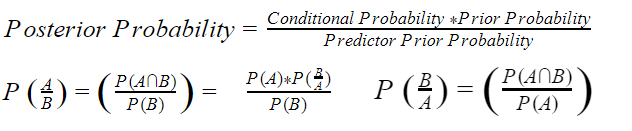
\includegraphics[scale=.7]{capture1.png}
        \caption{Bayesian Equation}
    \end{figure}
As this is a language processing problem, the Multinominal Naive Bayes approach was decided upon as it is the most common form of Naive Bayes used for machine learning predictions. Although there are various forms that the algorithm for this approach takes there are a few steps that all of them do follow that can detail the algorithm. First the data set is converted into a frequency table which will be done through the Bag of Words model, then create a likelihood table to find the probability, and finally use the Bayesian equation to calculate the probability under the condition that every word in every sentence is independent of each other. In a Multinominal approach, the distributions are parameterized by vectors $\theta_{y}$ with n features and $\theta_{yi}$ is the probability of feature i appearing in class y (P($x_{i}|_$y) [scikit-learn]). $\theta_{y}$ is estimated through relative frequency counting.


\section{Implementation}
\hspace{\parindent} To begin this Bayesian implementation we must begin by pre-processing the data. To understand what must be done to the data frame of metacritic user reviews (the only data set to go through pre-processing), we must first look at the shape of the fake review data frame that training and modeling will be completed on as if the shape of the data frames are not the same then they will be incompatible. Firstly, reviews that do not have a user comment are removed as they are of no use to the analysis without having words. While looking at the user comments it would beneficial to remove any reviews that do not have a unique comment, however our dataset did not have any non-unique entries. From here, attributes (username, platform, number) will be removed from the user metacritic reviews so that Dahlia's and Salminen's data share a shape as described in Table 2. The final change that needs to be made to allow both data frames to have the same shape is to cut Dahlia's csv file into multiple csv's (which will be combined in one output csv after processing them all) as Salminen's csv only has 40432 entries, whereas 283,982 entries. By splitting this will allow for the shape of (40432, 4), but that is not all that needs to be done for pre-processing. As this uses language processing the data needs to be scrubbed of punctuation and of 'stop words' (words that mark nouns, coordinate conjunction clauses, and occasional prepositions in sentences), which was done using NLTK's list of stop words. Finally with this done, the values of Dahlia's Comment attribute and Salminen's text attribute go through the process of feature extraction by using Scikitlearn's CountVectorizer to turn the data into a vector of terms being used. This allows for the creation of a bag of words from Salminen's data that will be used for determining what words are commonly used in spam reviews.\\

\begin{tabular}{ |p{6cm}|p{6cm}|  }
         \hline
           Dahlia's Attributes (user review data) &Salminen's Attibutes (training data)\\
         \hline
         Title&Category\\
         Userscore&rating\\
         label&label\\
         Comment&text\\
         \hline
\end{tabular}
\\ \\
\par Now that the data has been pre-processed and the shapes are a match training of the model can finally begin. To start training, the bag of words frequency table from Salminen's vectorized data frame will be used in comparison with the data given originally from Salminen. This data will be split so that 90 percent will be used for training and 10 percent will be used in testing what it learns from this with no random variability, which will then generate our likelihood tables. With this table finally being generated we are now ready to be fit for the Multinomial Naive Bayes equation, which will finally allow for reporting of what has been trained/tested thus far and also move forward with creating the predictions for the metacritic user reviews. When creating a prediction for the user reviews the predictions will be rounded, and then create an output csv of the data frame. From here, the output data frame is then used once more to create another data frame that is the mean of the legit reviews grouped by their titles. This data frame will finally be comparable to the Metacritic review scores in Deep Contractor's data set that will now be grouped similarly to how the output data frame was (sorted by title, obtaining the mean of duplicate game titles as Deep Contractor's data set would count the game on a console as a different game), and allowing for a conclusion on what type of difference using Naive Bayesian classifier had on the overall user scores.
\section{Results}
\hspace{\parindent} With the model finally trained on Salminen's dataset we are finally able to see the results of the training and testing periods. Figure 2 shows the classification reports for both our training and testing selections of Salminen's dataset, where in training the report believes it was accurate 88 percent of the time in it's overall classification of the data and an accuracy of 85. Although it would be better to have a higher accuracy through training the model more, it would require more training data, thus this will suffice for the sake of comparison. \\
    \begin{figure}[h]
        \centering
        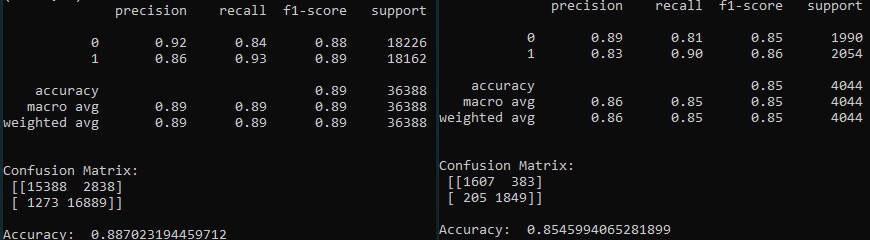
\includegraphics[scale=.6]{capture2.png}
        \caption{(Left) Report on Training (Right) Report on Testing}
    \end{figure}
\par From here, the trained model was then used on Dahlia's split csv's and recompiled into one output csv with an identifier of legit and spam reviews. This data is then re-organized and selected to create an average of the titles before classification and after the classification. The titles and ratings listed in Figure 3 describes a shortened list of the averages of each title. As seen in this figure, the classification was able to make a difference on many titles with the changes going anywhere from 0 to .4 on the overall score of titles.
\begin{figure}[h]
        \centering
        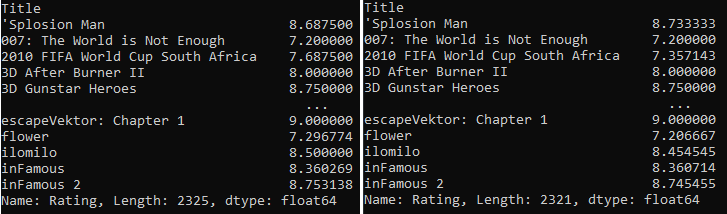
\includegraphics[scale=.75]{Averages.png}
        \caption{(Left) Average Before Classification (Right) Average After Classification}
    \end{figure}
On the other hand, there are a few games that noticeably have no changes at all. This can be caused by the fact that the majority of these titles that do not have any changes to them rather are not popular enough to have spam reviews attempt to sway the score, the title being a re-release that was not caught in conflict, or simply for unknown reasons. An example of this can be seen in 3D Gunstar Heroes which kept a user review average of 8.75. 3D Gunstar Heroes is a great example of these sorts of reasons as the game itself is a Nintendo 3DS 2015 re-release of Gunstar Heroes (originally published in 1993). The game on it's own is already quite obscure as the people who played the original have more than likely moved on from the series, while also being a re-release that got "3D" added along to the title because the game was released on the Nintendo 3DS with no new features besides being able to use the handheld's 3D capabilities. 
\par To have a better sample of the data to look at, let us look at a title that is considered to be revolutionary and one that is not so well remembered by the general gaming community. The Legend of Zelda: Ocarina of Time (1998) is a title that is well known for not only being one of the first three dimensional action titles, but also one of the most ground-breaking titles to show off how a title should function in this new dimension. Since it's release, not only has it been cherished by millions, but also has stayed at the top of Metacritic's highest rated games. On the other hand, there is Halo 5: Guardians (2015), a title that was notorious at it's release for numerous reasons that boil down to development being completed to meet the trends of titles at the time and not the demands of the fans who had been invested since the original Halo's release in 2001. That is not to say that Halo 5 does not have it's fair share of fans (and that Zelda: Ocarina of Time does not have people who dislike the game), but the general opinion of these releases do make a difference on the scores.
\begin{figure}[h]
        \centering
        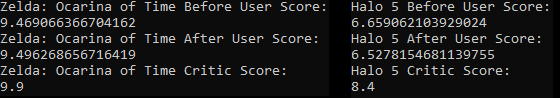
\includegraphics[scale=.8]{comps.png}
        \caption{Scoring of Titles}
    \end{figure}
As seen in Figure 4, the critic score for Zelda: Ocarina of Time is at a 9.9 and Halo 5's is sitting at an 8.4. When comparing Zelda's scores before and after classification, the score was bumped from 9.47 to a 9.5. When comparing Halo 5's scores before and after classification, the score went from 6.66 to 6.53. Although Zelda was able to get closer to the critic review score, Halo 5 only got farther away when attempting to remove spam reviews. Even with the changes from classification pointing to different ends of the spectrum, it is clear that the overwhelming majority of the reviews are legitimate and do not necessarily reflect the critic scores.
\par Although the data makes sense, it may not be the most reflective on a proper model to most efficiently remove spam reviews. Firstly, this can be caused by the ~88 percent accuracy in training. Having a higher accuracy and precision will give better results, however that would require more time and training data sets of the same shape (meaning more fake reviews with scores) to allow for this. Another issue is also the training dataset used; the reviews in Salminen's dataset were reviews of various types of products, and as a result the bag of words generated from this dataset does not necessarily reflect the words used in video game reviews. The final issue is in Dahlia's dataset of Metacritic User Reviews, where many of the reviews are not in english and as a result can cause some false positives/negatives. Figures 5 and 6 shows these issues, where the words used in both data sets do not have too many that overlap, and figure 6 having non-english characters that should have been classified as garbage appearing.
\begin{figure}[h]
        \centering
        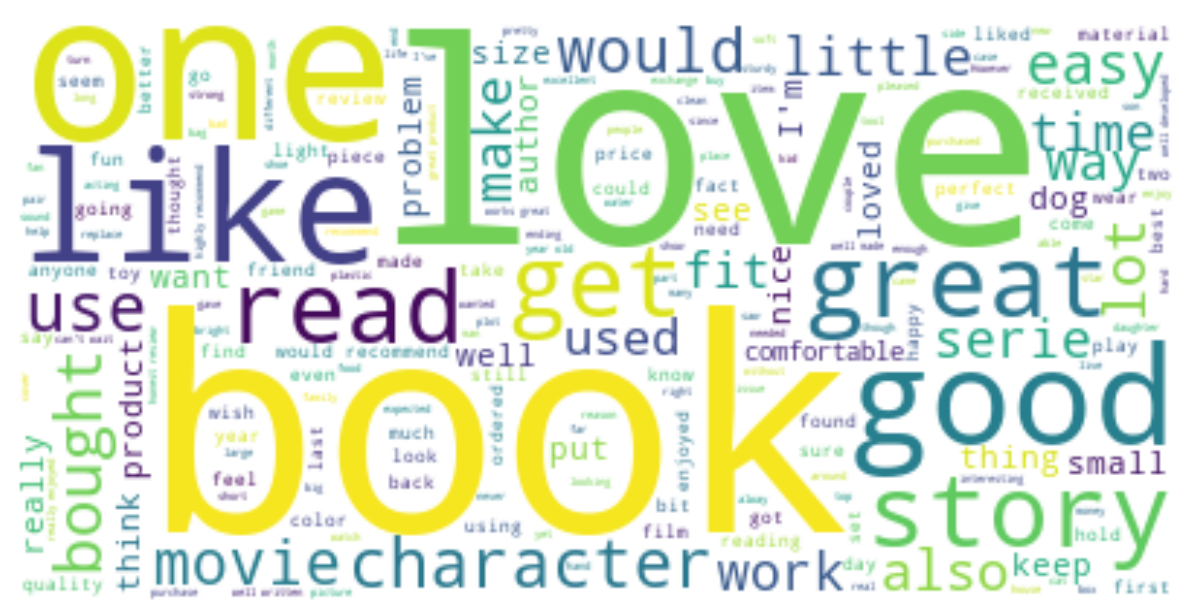
\includegraphics[scale=.4]{trainWords.png}
        \caption{Word Cloud for Training Data}
    \end{figure}
\begin{figure}[h]
        \centering
        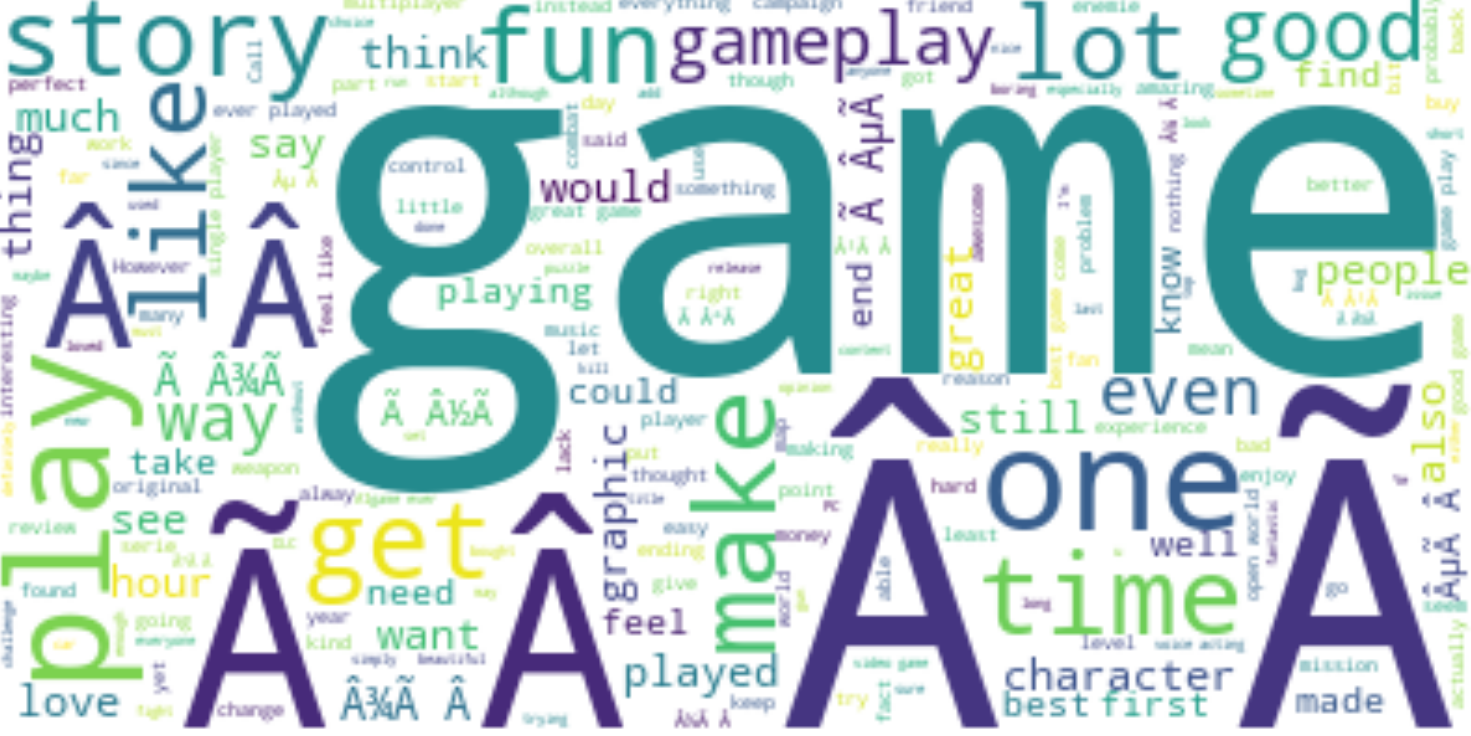
\includegraphics[scale=.3]{testWords.png}
        \caption{Word Cloud for User Review Data}
    \end{figure}
    \\
\section{Conclusion}
\hspace{\parindent} Naive Bayes Classification is a great way to be able to create predictions upon natural language processing problems by creating a frequency table to create a likelihood table to find probabilities, and use the Bayesian equation to make predictions. In the model created here, training data of real and fake consumer product reviews were used to make predictions on video game reviews on Metacritic to determine authenticity. The majority of user reviews were deemed to not be spam, which is a realistic expectation for this classification even though it may not be the most accurate. If this project was continued, it can be expected that the accuracy would be able to be improved over time as the Naive Bayes Classification allows for updating to better the model. This would further be the case if there were publicly available datasets similar to Salminen's training dataset, but exclusively for video games to be able to obtain a bag of words more appropriate to the words typical for a video game review.
\pagebreak
\section{References}
\begin{itemize}
    \item Kaggle Dataset - Top Video Games 1995-2021 Metacritic by Deep Contractor:\\ https://www.kaggle.com/deepcontractor/top-video-games-19952021-metacritic/version/4
    \item Kaggle Dataset - Metacritic Video Game Comments by Dahlia:\\ https://www.kaggle.com/dahlia25/metacritic-video-game-comments/activity
    \item OSFHome - Fake Reviews Dataset https://osf.io/tyue9/
    \item Email Spam Detection Using Python &amp; Machine Learning. YouTube. (2019, August 7). Retrieved April 1, 2022, \\from https://www.youtube.com/watch?v=cNLPt02RwF0&ab\textunderscore channel=ComputerScience
    \item Common Spam Filtering Techniques . Process Software. (n.d.). Retrieved April 26, 2022, from https://www.process.com/products/pmas/whitepapers/explanation\textunderscore filter \textunderscore techniques.pdf
    \item Great Learning Team. (2022, March 7). Multinomial naive Bayes explained. GreatLearning Blog Retrieved April 25, 2022, from \\ https://www.mygreatlearning.com/blog/multinomial-naive-bayes-explained/ 
    \item 1.9 Naive Bayes. Scikit Learn. (n.d.). Retrieved April 25, 2022, from  https://scikit-learn.org/stable/modules/naive\textunderscore bayes.html
\end{itemize}
\end{document}
